\documentclass[a4paper,14pt]{article}
\usepackage[warn]{mathtext} %для поддержки кириллицы в формулах
\usepackage{amsmath} %основной пакет для формул
\usepackage[utf8x]{inputenc}
\usepackage[T1,T2A]{fontenc}
\usepackage[russian]{babel}
\usepackage{hyperref}
\usepackage{indentfirst}
\usepackage{listings}
\usepackage{color}
\usepackage{here}
\usepackage{array}
\usepackage{multirow}
\usepackage{graphicx}

\usepackage{caption}
\renewcommand{\lstlistingname}{Программа} % заголовок листингов кода

\usepackage{listings}
\lstset{ %
extendedchars=\true,
keepspaces=true,
language=bash,					% choose the language of the code
basicstyle=\footnotesize,		% the size of the fonts that are used for the code
numbers=left,					% where to put the line-numbers
numberstyle=\footnotesize,		% the size of the fonts that are used for the line-numbers
stepnumber=1,					% the step between two line-numbers. If it is 1 each line will be numbered
numbersep=5pt,					% how far the line-numbers are from the code
backgroundcolor=\color{white},	% choose the background color. You must add \usepackage{color}
showspaces=false				% show spaces adding particular underscores
showstringspaces=false,			% underline spaces within strings
showtabs=false,					% show tabs within strings adding particular underscores
frame=single,           		% adds a frame around the code
tabsize=2,						% sets default tabsize to 2 spaces
captionpos=b,					% sets the caption-position to bottom
breaklines=true,				% sets automatic line breaking
breakatwhitespace=false,		% sets if automatic breaks should only happen at whitespace
escapeinside={\%*}{*)},			% if you want to add a comment within your code
postbreak=\raisebox{0ex}[0ex][0ex]{\ensuremath{\color{red}\hookrightarrow\space}}
}

\usepackage[left=2cm,right=2cm,
top=2cm,bottom=2cm,bindingoffset=0cm]{geometry}


\begin{document}	% начало документа

\begin{titlepage}	% начало титульной страницы

	\begin{center}		% выравнивание по центру

		\large Санкт-Петербургский политехнический университет Петра Великого\\
		\large Институт компьютерных наук и технологий \\
		\large Кафедра компьютерных систем и программных технологий\\[1cm]
		
		\includegraphics[scale=0.7]../pics/spbpu.jpg}\\[2cm]
		
		\huge Реферат по компьютерной алгебре\\[0.5cm] % название работы, затем отступ 0,5см
		\huge Алгоритмы сжатия изображений\\[3cm]

	\end{center}	
	
	\begin{flushright} % выравнивание по правому краю
		\begin{minipage}{0.25\textwidth} % врезка в половину ширины текста
			\begin{flushleft} % выровнять её содержимое по левому краю

				\large\textbf{Студенты:}\\
				\large В.В. ~Дьячков\\
				\large А.А. ~Жуйков\\
				\large А.Ю. ~Ламтев\\
				\large Ю.И. ~Леженин\\
				\large {Группа:} 13501/4\\
				
				\large \textbf{Преподаватель:}\\
				\large И.А. ~Малышев\\

			\end{flushleft}
		\end{minipage}
	\end{flushright}
	
	\vfill % заполнить всё доступное ниже пространство

	\begin{center}
	\large Санкт-Петербург\\
	\large \the\year % вывести дату
	\end{center} % закончить выравнивание по центру
\thispagestyle{empty} % не нумеровать страницу
\end{titlepage} % конец титульной страницы

\vfill % заполнить всё доступное ниже пространство



% Содержание
\hypertarget{toc}
\tableofcontents
\newpage


\section*{\hyperlink{toc}{Введение}}
\addcontentsline{toc}{section}{Введение}

Сейчас мы живем в информационном обществе, и нас окружает огромный объем информации в том числе и графической. Наверно хоть раз вы отправляли картинку своему приятелю в социальной сети. Цифровое изображение при хранении занимает большие объемы памяти. Так растровое изображение размером 1024 на 1024 пикселей с глубиной цвета 24 бит занимает 3 Мб. Понятно, что хранение и передача изображений в таком виде является весьма трудоёмкой задачей. Поэтому задача представления изображений в компактной форме (сжатие данных) является весьма актуальной. При этом должны быть разработаны алгоритмы как для кодирования, так и для декодирования (восстановления) изображений. 
	
Первыми для архивации изображений стали применяться привычные алгоритмы. Те, что использовались и используются в системах резервного копирования, при создании дистрибутивов и т.п. Эти алгоритмы архивировали информацию без изменений. Однако основной тенденцией в последнее время стало использование новых классов изображений. Старые алгоритмы перестали удовлетворять требованиям, предъявляемым к архивации. Многие изображения практически не сжимались, хотя “на взгляд” обладали явной избыточностью. Это привело к созданию нового типа алгоритмов — сжимающих с потерей информации. Как правило, коэффициент архивации и, следовательно, степень потерь качества в них можно задавать. При этом достигается компромисс между размером и качеством изображений.
	
Идея, лежащая в основе всех алгоритмов сжатия с потерями, довольно проста: на первом этапе удалить несущественную информацию, а на втором этапе к оставшимся данным применить наиболее подходящий алгоритм сжатия без потерь. Основные сложности заключаются в выделении этой несущественной информации. Подходы здесь существенно различаются в зависимости от типа сжимаемых данных. Для звука чаще всего удаляют частоты, которые человек просто не способен воспринять, уменьшают частоту дискретизации, а также некоторые алгоритмы удаляют тихие звуки, следующие сразу за громкими, для видеоданных кодируют только движущиеся объекты, а незначительные изменения на неподвижных объектах просто отбрасывают. Методы выделения несущественной информации на изображениях будут подробно рассмотрены далее.

\section*{\hyperlink{toc}{Методы и алгоритмы сжатия}}
\addcontentsline{toc}{section}{Методы и алгоритмы сжатия}

\subsection*{\hyperlink{toc}{Цветовое пространство $YC_bC_r$ и цветовая субдискретизация}}
\addcontentsline{toc}{subsection}{Цветовое пространство $YC_bC_r$ и цветовая субдискретизация}

% http://sernam.ru/cod_7.php
Известно, что органы зрения человека менее чувствительны к цвету предметов, чем к их яркости. В цветовом пространстве RGB все три компонента считаются одинаково важными, и они обычно сохраняются с одинаковым разрешением. Однако можно отобразить цветовое изображение более эффективно, отделив светимость от цветовой информации и представив ее с большим разрешением, чем цвет. Поэтому цветовое пространство YCbCr и его вариации является популярным методом эффективного представления цветных изображений. 

Буква Y в таких цветовых пространствах обозначает компоненту светимость, которая вычисляется как взвешенное усреднение компонент R, G и B по следующей формуле: 

\begin{displaymath}
	Y = k_rR + k_gG + k_bB
\end{displaymath}

$k$ - соответствующий весовой множитель.

Остальные цветовые компоненты по существу определяются в виде разностей между светимостью Y и компонентами R, G и B: 

\begin{center}
	$C_b = B - Y$ 

	$C_r = C - Y$ 

	$C_g = G - Y$ 
\end{center}

%картинка 1

Число $C_b+C_r+C_g$ является постоянным, поэтому только две из трех хроматических компонент необходимо хранить, а третью можно вычислить на их основе. Чаще всего в качестве две искомых цветовых компонент используют $C_b$ и $C_r$. 

%картинка 2

Преобразование цветового пространства дает дополнительный эффект при сжатии цветных изображений. При этом алгоритмы сжатия сначала преобразуют исходное цветовое пространство из RGB в $YC_bC_r$, сжимают, а затем при восстановлении обратно преобразуют изображение в цветовое пространство RGB. Обычно преобразованное изображение подвергается цветовой субдескретизации для дальнейшего сжатия.

%https://ru.wikipedia.org/wiki/%D0%A6%D0%B2%D0%B5%D1%82%D0%BE%D0%B2%D0%B0%D1%8F_%D1%81%D1%83%D0%B1%D0%B4%D0%B8%D1%81%D0%BA%D1%80%D0%B5%D1%82%D0%B8%D0%B7%D0%B0%D1%86%D0%B8%D1%8F
Цветовая субдискретизация — технология кодирования изображений со снижением цветового разрешения, при которой частота выборки цветоразностных сигналов может быть меньше частоты выборки яркостного сигнала. Основана на особенности человеческого зрения, выраженной большей чувствительностью к перепадам яркости, чем цвета. 

Структура дискретизации сигнала обозначается как соотношение между тремя частями X:a:b (например, 4:2:2, рис. \ref{pic:chroma_subsampling} ), описывающими число выборок яркостных и цветоразностных сигналов. Этими частями являются:

\begin{itemize}
	
	\item X — частота дискретизации яркостного канала, выраженная коэффициентом базовой частоты (ширина макропикселя)
	
	\item a — число выборок цветоразностных сигналов ($C_r$, $C_b$) в горизонтальном направлении в первой строке
	
	\item b — число (дополнительных) выборок цветоразностных сигналов ($C_r$, $C_b$) во второй строке
	
\end{itemize}


%картинка 3

Цветовая субдискретизация является важным способом снижения скорости цифрового потока видеоданных (цифровое сжатие видеоинформации). Используется в системах аналогового и цифрового телевидения, цифровой видеозаписи и алгоритмах сжатия изображений, таких как JPEG.

\subsection*{\hyperlink{toc}{Квантование и дискретизация}}
\addcontentsline{toc}{subsection}{Квантование и дискретизация}

%https://habrahabr.ru/post/251417/
С процессом квантования и дискретизации связано понятие визуальной избыточности. Значительная часть информации на изображении не может быть воспринята человеком: например, человек способен замечать незначительные перепады яркости, но гораздо менее чувствителен к цветности. Также, начиная с определённого момента, повышение точности дискретизации не влияет на визуальное восприятие изображения. Таким образом, некоторая часть информации может быть удалена без ухудшения визуального качества. Такую информацию называют визуально избыточной.

Наиболее удобным с точки зрения организации обработки и естественным способом дискретизации является представление сигналов в виде выборки их значений (отсчетов) в отдельных, регулярно расположенных точках. Такой способ называют растрированием, а последовательность узлов, в которых берутся отсчеты – растром. Интервал, через который берутся значения непрерывного сигнала называется шагом дискретизации. Обратная шагу величина называется частотой дискретизации.

Самым простым способом удаления визуальной избыточности является уменьшение точности дискретизации, но на практике этот способ можно применять только для изображений с простой структурой, т.к. искажения, возникающие на сложных изображениях, слишком заметны.(рис. \ref{pic:shakal})

%картинка 4

Для удаления избыточной информации чаще уменьшают точность квантования, но нельзя уменьшать её бездумно, т.к. это приводит к резкому ухудшению качества изображения. Предположим, что изображение представлено в цветовом пространстве RGB, результаты кодирования этого изображения с пониженной точностью квантования представлены на рис. \ref{pic:levels_of_quantization}.

%картинка 5

Не следует путать квантование с дискретизацией (и, соответственно, шаг квантования с частотой дискретизации). При дискретизации изменяющаяся во времени величина (сигнал) замеряется с заданной частотой (частотой дискретизации), таким образом, дискретизация разбивает сигнал по временной составляющей. Квантование же приводит сигнал к заданным значениям, то есть, разбивает по уровню сигнала.

Внимательно изучив полученные изображения, можно заметить, что на сжатых изображениях возникают отчётливые ложные контуры, которые значительно ухудшают визуальное восприятие. Существуют методы, основанные на переносе ошибки квантования в следующий пиксел, позволяющие значительно уменьшить или даже совсем удалить эти контуры, но они приводят к зашумлению изображения и появлению зернистости. Перечисленные недостатки сильно ограничивают прямое применение квантования для сжатия изображений.

Большинство современных методов удаления визуально избыточной информации используют сведения об особенностях человеческого зрения. Всем известна различная чувствительность человеческого глаза к информации о цветности и яркости изображения.

%картинка 6

Как видно на рис. \ref{pic:quantization}, глубина квантования цветоразностных сигналов может быть понижена с 256 до 32 уровней с минимальными визуальными изменениями. В то же время потери в I и Q составляющих весьма существенны. Несмотря на простоту описанных методов, в чистом виде они применяются редко, чаще всего они служат одним из шагов более эффективных алгоритмов.

\subsection*{\hyperlink{toc}{Вейвлет сжатие}}
\addcontentsline{toc}{subsection}{Вейвлет сжатие}

%source: https://habrahabr.ru/post/251417/
Вейвлеты – математические функции, предназначенные для анализа частотных компонент данных. В задачах сжатия информации вейвлеты используются сравнительно недавно, тем не менее исследователям удалось достичь впечатляющих результатов.
В отличие от рассмотренных выше преобразований, вейвлеты не требуют предварительного разбиения исходного изображения на блоки, а могут применяться к изображению в целом. В данном разделе вейвлет сжатие будет пояснено на примере довольно простого вейвлета Хаара.
Для начала рассмотрим преобразование Хаара для одномерного сигнала. Пусть есть набор S из n значений, при преобразовании Хаара каждой паре элементов ставится в соответствие два числа: полусумма элементов и их полуразность. Важно отметить, что это
 преобразование обратимо: т.е. из пары чисел можно легко восстановить исходную пару. На рис. \ref{pic:wavelet_example} показан пример одномерного преобразования Хаара.

%картинка 7

Видно, что сигнал распадается на две составляющее: приближенное значение исходного (с уменьшенным в два раза разрешением) и уточняющую информацию.
Двумерное преобразование Хаара – простая композиция одномерных преобразований. Если исходные данные представлены в виде матрицы, то сначала выполняется преобразование для каждой строки, а затем для полученных матриц выполняется преобразование для каждого столбца. На рис. \ref{pic:wavelet_compression} показан пример двумерного преобразования Хаара.

%картинка 8

Цвет пропорционален значению функции в точке (чем больше значение, тем темнее). В результате преобразования получается четыре матрицы: одна содержит аппроксимацию исходного изображения (с уменьшенной частотой дискретизации), а три остальных содержат уточняющую информацию.
Сжатие достигается путём удаления некоторых коэффициентов из уточняющих матриц. На рис. \ref {pic:wavelet_uncompression} продемонстрирован процесс восстановления и само восстановленное изображение после удаления из уточняющих матриц малых по модулю коэффициентов:

%картинка 9

Очевидно, что представление изображения с помощью вейвлетов позволяет добиваться эффективного сжатия, сохраняя при этом визуальное качество изображения. Существуют и другие вейвлеты, с помощью которых производится сжатие изображений.

\subsection*{\hyperlink{toc}{Алгоритм сжатия RLE}}
\addcontentsline{toc}{subsection}{Алгоритм сжатия RLE}

%source: https://habrahabr.ru/post/251417/
Все алгоритмы серии RLE основаны на очень простой идее: повторяющиеся группы элементов заменяются на пару (количество повторов, повторяющийся элемент). 

Рассмотрим этот алгоритм на примере последовательности бит. В этой последовательности будут чередовать группы нулей и единиц. Причём в группах зачастую будет более одного элемента. Тогда последовательности 11111 000000 11111111 00 будет соответствовать следующий набор чисел 5 6 8 2. Эти числа обозначают количество повторений (отсчёт начинается с единиц), но эти числа тоже необходимо кодировать. Будем считать, что число повторений лежит в пределах от 0 до 7 (т.е. нам хватит 3 бит для кодирования числа повторов). Тогда рассмотренная выше последовательность кодируется следующей последовательностью чисел 5 6 7 0 1 2. Легко подсчитать, что для кодирования исходной последовательности требуется 21 бит, а в сжатом по методу RLE виде эта последовательность занимает 18 бит.

Хоть этот алгоритм и очень прост, но эффективность его сравнительно низка. Более того, в некоторых случаях применение этого алгоритма приводит не к уменьшению, а к увеличению длины последовательности. Для примера рассмотрим следующую последовательность 111 0000 11111111 00. Соответствующая ей RL-последовательность выглядит так: 3 4 7 0 1 2. Длина исходной последовательности – 17 бит, длина сжатой последовательности – 18 бит.

Этот алгоритм наиболее эффективен для чёрно-белых изображений. Также он часто используется, как один из промежуточных этапов сжатия более сложных алгоритмов.

\subsection*{\hyperlink{toc}{Алгоритм сжатия LZW}}
\addcontentsline{toc}{subsection}{Алгоритм сжатия LZW}

Идея, лежащая в основе словарных алгоритмов, заключается в том, что происходит кодирование цепочек элементов исходной последовательности. При этом кодировании используется специальный словарь, который получается на основе исходной последовательности. 

Существует целое семейство словарных алгоритмов, но мы рассмотрим наиболее распространённый алгоритм LZW, названный в честь его разработчиков Лепеля, Зива и Уэлча. 

Словарь в этом алгоритме представляет собой таблицу, которая заполняется цепочками кодирования по мере работы алгоритма. При декодировании сжатого кода словарь восстанавливается автоматически, поэтому нет необходимости передавать словарь вместе с сжатым кодом. 

Рассмотрим пример сжатия алгоритмом. Будем сжимать строку \textbf{кукушкакукушонкукупилакапюшон}. Предположим, что словарь будет вмещать 32 позиции, а значит, каждый его код будет занимать 5 бит.

Сначала словарь инициализируется всеми одноэлементными цепочками, т.е. первые строки словаря представляют собой алфавит, в котором мы производим кодирование. Изначально словарь будете заполнен как на рис. \ref{pic:lzw:dictionary}

%картинка 10

При сжатии происходит поиск наиболее длинной цепочки уже записанной в словарь. Каждый раз, когда встречается цепочка, ещё не записанная в словарь, она добавляется туда, при этом выводится сжатый код, соответствующий уже записанной в словаре цепочки(рис. \ref{pic:lzw:result}).

%картинка 11 

В теории на размер словаря не накладывается никаких ограничений, но на практике есть смысл этот размер ограничивать, так как со временем начинаются встречаться цепочки, которые больше в тексте не встречаются. Кроме того, при увеличении размеры таблицы вдвое мы должны выделять лишний бит для хранения сжатых кодов.
  
\subsection*{\hyperlink{toc}{Алгоритм Хаффмана}}
\addcontentsline{toc}{subsection}{Алгоритм Хаффмана}

Алгоритм Хаффмана позволяет строить префиксные коды. Можно рассматривать префиксные коды как пути на двоичном дереве: прохождение от узла к его левому сыну соответствует 0 в коде, а к правому сыну – 1. Если мы пометим листья дерева кодируемыми символами, то получим представление префиксного кода в виде двоичного дерева.\\
Опишем алгоритм построения дерева Хаффмана и получения кодов Хаффмана.
\begin{enumerate}

	\item Символы входного алфавита образуют список свободных узлов. Каждый лист имеет вес, который равен частоте появления символа;
	\item Выбираются два свободных узла дерева с наименьшими весами;
	\item Создается их родитель с весом, равным их суммарному весу;
	\item Родитель добавляется в список свободных узлов, а двое его детей удаляются из этого списка;
	\item Одной дуге, выходящей из родителя, ставится в соответствие бит 1, другой — бит 0;
	\item Шаги, начиная со второго, повторяются до тех пор, пока в списке свободных узлов не останется только один свободный узел. Он и будет считаться корнем дерева.

\end{enumerate}


\subsection*{\hyperlink{toc}{Дискретное косинусное преобразование}}
\addcontentsline{toc}{subsection}{Дискретное косинусное преобразование}
Дискретное косинусное преобразование представляет собой разновидность преобразования Фурье и, также как и последнее, имеет обратное преобразование (ОДКП). Если рассматривать изображение как совокупность пространственных волн, где оси X~и~Y соответствуют ширине и высоте картинки, а по оси Z откладываются значения цвета соответствующих пикселей, то можно перейти от пространственного представления картинки к ее спектральному представлению и обратно. ДКП преобразует матрицу пикселей размера $N \times N$ в матрицу частотных коэффициентов соответствующего размера.

Как видно на рис. \ref{pic:cosine_tranform:matrix}, в получаемой матрице низкочастотные компоненты расположены ближе к левому верхнему углу, а более высокочастотные смещаются вправо вниз. В связи с тем, что основная часть графических образов на экране состоит из низкочастотной информации, используя полученную матрицу можно дифференцированно отбрасывать наименее важную информацию с минимальными визуальными потерями. Таким образом ДКП позволяет выбрать информацию, которую можно безболезненно отбросить, не внося серьезных искажений в картинку. Трудно представить, как можно было бы выполнить эту задачу на исходном изображении.

Вычисление одного элемента результирующей матрицы требует $O(N^2)$ времени, поэтому почти невозможно выполнить преобразование всей матрицы целиком. Группа разработчиков JPEG предложила оптимальный вариант решения этой проблемы: разбивать исходную матрицу на квадраты стандартного размера $8\times8$ и выполнять преобразование каждого из них. Использование блоков большего размера позволит улучшить качество сжатия, но не до бесконечности, так как слишком мала вероятность того, что сильно отдаленные точки похожи друг на друга.

Стоит отметить, что в ходе вычислений используется только 32 заранее вычисленных значения косинусов, что позволяет заметно увеличить скорость работы преобразования. Это уже, несомненно, приводит к частичной потери информации, но ее объемы относительно несущественны.

\section*{\hyperlink{toc}{Выводы}}
\addcontentsline{toc}{section}{Выводы}

Всё круто!!!

\section*{\hyperlink{toc}{Источники}}
\addcontentsline{toc}{section}{Источники}

\begin{itemize}

	\item\href{https://habrahabr.ru/post/116697}{https://habrahabr.ru/post/116697}
	\item\href{https://habrahabr.ru/post/251417/}{https://habrahabr.ru/post/251417/}
	\item\href{https://habrahabr.ru/post/144200/}{https://habrahabr.ru/post/144200/}
	\item\href{https://ru.wikipedia.org/wiki/%D0%A6%D0%B2%D0%B5%D1%82%D0%BE%D0%B2%D0%B0%D1%8F_%D1%81%D1%83%D0%B1%D0%B4%D0%B8%D1%81%D0%BA%D1%80%D0%B5%D1%82%D0%B8%D0%B7%D0%B0%D1%86%D0%B8%D1%8F}{https://ru.wikipedia.org/wiki/Цветовая\_субдискретизация}
	\item\href{http://sernam.ru/cod_7.php}{http://sernam.ru/cod\_7.php}
	\item Конспект лекций по Дискретной математике Митиной Т.М.
	\item\href{https://github.com/ejiek/latex_templates}{Репозиторий с шаблонами для \LaTeX}
	
\end{itemize}
\newpage

\section*{\hyperlink{toc}{Приложение}}
\addcontentsline{toc}{section}{Приложение}

\begin{figure}[H]
	\begin{center}
		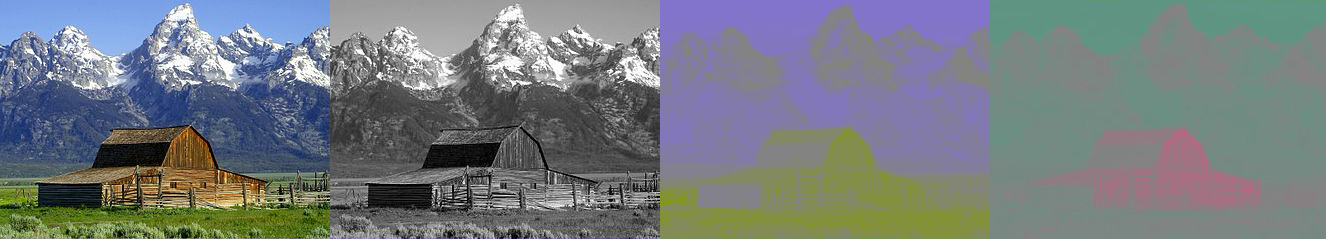
\includegraphics[scale=0.35]{../pics/YCbCr/YCbCr_separation_h.jpg}
		\caption{Цветное изображение и его компоненты Y, $C_B$ и $C_R$} 
		\label{pic:YCbCr:separation}
	\end{center}
\end{figure}

\begin{figure}[H]
	\begin{center}
		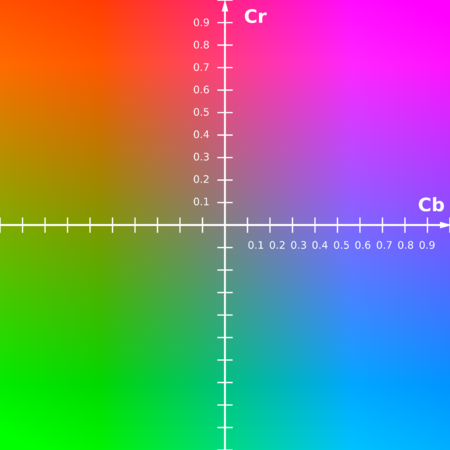
\includegraphics[scale=0.5]{../pics/YCbCr/YCbCr.png}
		\caption{Плоскость $YC_bC_r$ при постоянной яркости Y = 0.5} 
		\label{pic:YCbCr:separation}
	\end{center}
\end{figure}

\begin{figure}[H]
	\begin{center}
		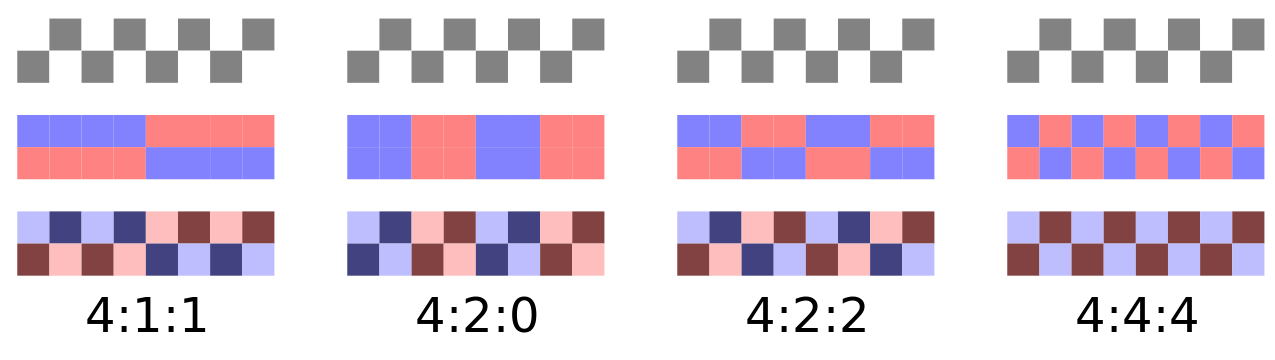
\includegraphics[scale=0.35]{../pics/chroma_subsampling/chroma_subsampling_ratios.png}
		\caption{Форматы субдискретизации} 
		\label{pic:chroma_subsampling}
	\end{center}
\end{figure}

\begin{figure}[H]
	\begin{center}
		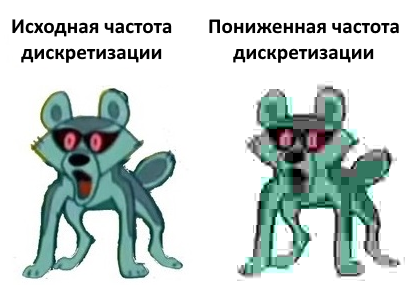
\includegraphics[scale=0.9]{../pics/quantization/shakal.png}
		\caption{Уменьшение точности дискретизации} 
		\label{pic:shakal}
	\end{center}
\end{figure}

\begin{figure}[H]
	\begin{center}
		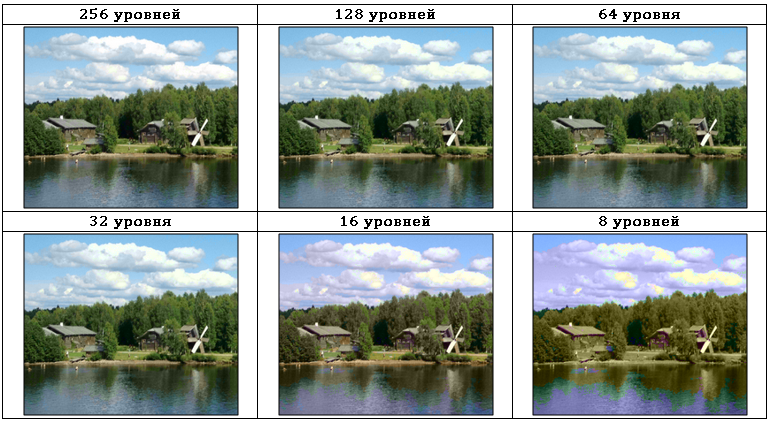
\includegraphics[scale=0.85]{../pics/quantization/levels_of_quantization.png}
		\caption{Уменьшение глубины квантования} 
		\label{pic:levels_of_quantization}
	\end{center}
\end{figure}

\begin{figure}[H]
	\begin{center}
		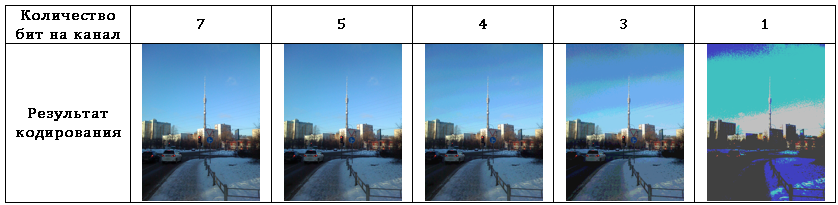
\includegraphics[scale=0.75]{../pics/quantization/quantization.png}
		\caption{Различная глубина квантования цветоразностных сигналов IQ} 
		\label{pic:quantization}
	\end{center}
\end{figure}

\begin{figure}[H]
	\begin{center}
		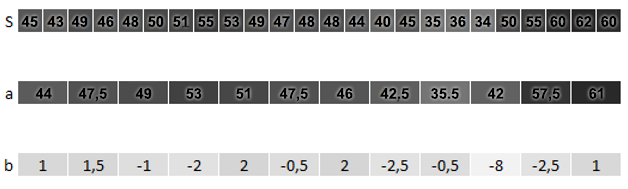
\includegraphics[scale=0.9]{../pics/wavelet/example.png}
		\caption{Пример для одномерного пространства} 
		\label{pic:wavelet_example}
	\end{center}
\end{figure}

\begin{figure}[H]
	\begin{center}
		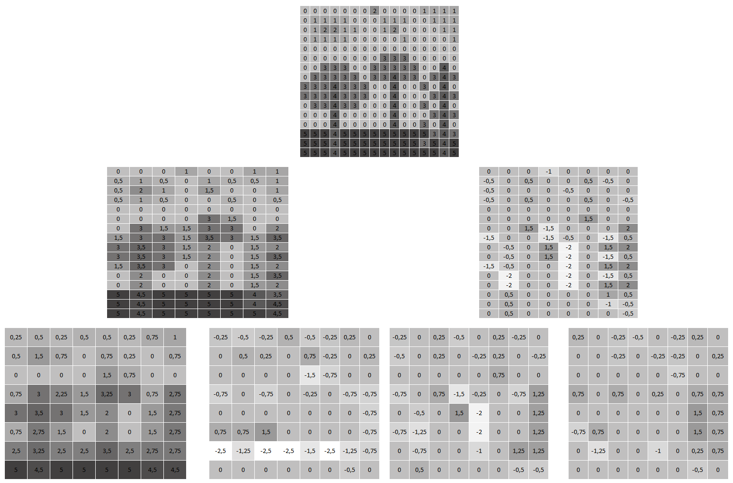
\includegraphics[scale=0.7]{../pics/wavelet/compression.png}
		\caption{Процесс сжатия} 
		\label{pic:wavelet_compression}
	\end{center}
\end{figure}

\begin{figure}[H]
	\begin{center}
		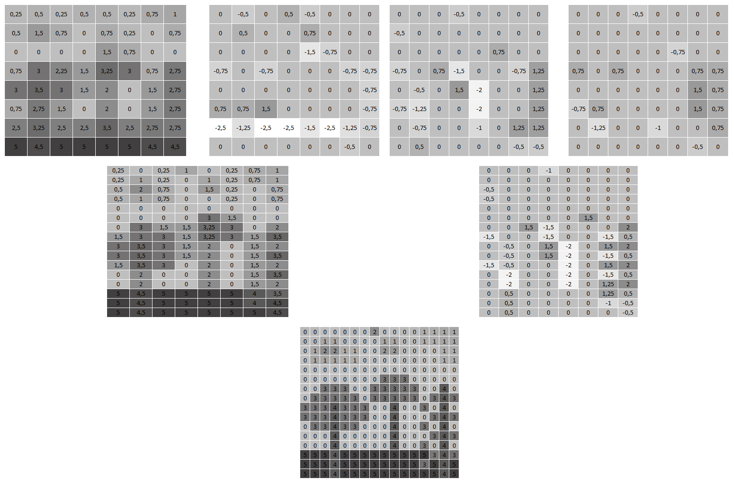
\includegraphics[scale=0.7]{../pics/wavelet/uncompression.png}
		\caption{Процесс восстановления} 
		\label{pic:wavelet_uncompression}
	\end{center}
\end{figure}

\begin{figure}[H]
	\begin{center}
		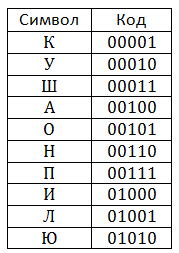
\includegraphics[scale=1]{../pics/LZW/dictionary.png}
		\caption{Начальный словарь} 
		\label{pic:lzw:dictionary}
	\end{center}
\end{figure}

\begin{figure}[H]
	\begin{center}
		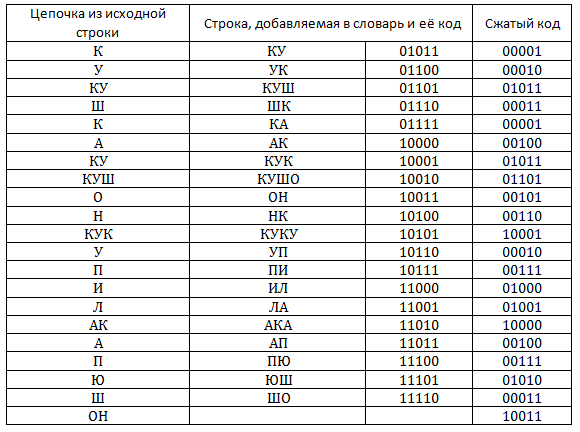
\includegraphics[scale=1]{../pics/LZW/result.png}
		\caption{Процесс и результат кодирования}
		\label{pic:lzw:result}
	\end{center}
\end{figure}
\begin{figure}[H]
	\begin{center}
		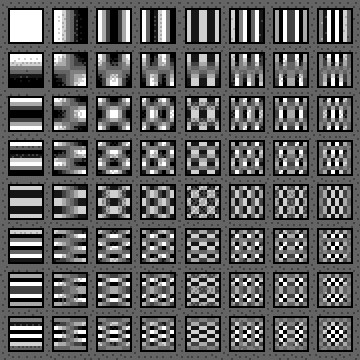
\includegraphics[scale=1]{../pics/cosine_transform/matrix.png}
		\caption{Матрица, полученная ДКП}
		\label{pic:cosine_tranform:matrix}
	\end{center}
\end{figure}


\end{document}
